\chapter{Große Abbildungen}
Im Folgenden sind größere Abbildungen dargestellt, die eine ganze Seite oder eine Doppelseite einnehmen.

\noindent Tabelle~\ref{tbl:kommandos} führt eine Auswahl der möglichen Befehle für den Kaffeevollautomaten auf.
Die vollständige Liste befindet sich unter \texttt{JuraCoffeeMemory/result/commands.txt}.

\noindent Abbildung~\ref{fig:Speicherschema} zeigt schematisch den Speicher des Kaffeevollautomaten.
Der \ac{EEPROM} und der \ac{RAM} sind in jeweils 16 Zeilen zeilenweise dargestellt.

\noindent Tabelle~\ref{tbl:RAM1} und Tabelle~\ref{tbl:RAM2} stellen spaltenweise die Bit-Änderungen für je eine Meldung oder Funktion im \ac{RAM} dar.

\noindent Abbildung~\ref{fig:API-EEPROM} und Abbildung~\ref{fig:API-RAM} zeigen die abgefragten Wörter und Bytes für die Ausgabe der \ac{API}.

\noindent Tabelle~\ref{tbl:Displaysymbole} stellt den verfügbare Zeichensatz für das Display dar.
Gleichzeitig werden die dafür nötigen \ac{ASCII} Kommando-Eingaben aufgeführt.

\begin{tuhhtable}
  \footnotesize\centering
  \begin{tabular}[tp]{L{.22\textwidth}L{.48\textwidth}L{.18\textwidth}}
%
  \THc{1}{c}{Kommando} & \THc{1}{c}{Beschreibung} & \THc{1}{c}{Rückgabewert} \\
%
  \TRx{3}{l}{Betriebszustand (AN:<id>)}\\
  \abovebodyrule
  AN:01    & Einschalten        & ok:    \\\TRc
  AN:02    & Ausschalten        & ok:    \\
  AN:03    & Display Test       & ok:    \\\TRc
  AN:<id>  & u.v.m.             & ok:    \\
  \belowbodyrule
%
  \TRx{3}{l}{Bezugstaste (FA:<id>)}\\
  \abovebodyrule
  FA:02    & Gerät spülen       & ok:    \\\TRc
  FA:0C    & Spezialkaffee      & ok:    \\
  FA:<id>  & u.v.m.             & ok:    \\\TRc
  \belowbodyrule
%
  \TRx{3}{l}{Steuerungskomponenten (FN:<id>)}\\
  \abovebodyrule
  FN:<id>  & Pumpen, Heizung, u.v.m & ok:    \\\TRc
  \belowbodyrule
%
  \TRx{3}{l}{Eingabestatus*}\\
  \abovebodyrule
  IC:      & Eingaben auslesen* &        \\\TRc
  \belowbodyrule
%
  \TRx{3}{l}{Spiele Musik (easter egg)*}\\
  \abovebodyrule
  PM:      & Play music*        &        \\\TRc
  \belowbodyrule
%
  \TRx{3}{l}{Speicherzugriff}\\
  \abovebodyrule
  RE:<address> & Liest 2 Byte EEPROM Speicher   & re:[0000-FFFF] \\\TRc
  WE:<address>,<value> & Schreibt 2 Byte in EEPROM & ok:         \\
  RT:<address> & Liest eine Zeile EEPROM        & rt:[0-F 64x]   \\\TRc
  RR:<address> & Liest eine Zeile RAM           & rr:[0-F 32x]   \\
  \belowbodyrule
%
  \TRx{3}{l}{Sperrung}\\
  \abovebodyrule
  ?M3      & Aktiviert den Inkassomodus         & ?ok            \\\TRc
  ?M1      & Deaktiviert den Inkassomodus       & ?ok            \\
  \belowbodyrule
%
  \TRx{3}{l}{Display}\\
  \abovebodyrule
  ?D0      & Standard Displaytext zurück setzen & ?ok            \\\TRc
  ?D1[A-Z 8-11x] & Displaytext Zeile 1          & ?ok            \\
  ?D2[A-Z 8-11x] & Displaytext Zeile 2          & ?ok            \\\TRc
  \belowbodyrule
%
  \TRx{3}{l}{Aktion an der Kaffeemaschine}\\
  \abovebodyrule
           & 1 kleiner Kaffee (Produkt 1)       & ?PAE         \\\TRc
           & 2 kleine Kaffees (Produkt 2)       & ?PAF         \\
           & 1 großer Kaffee  (Produkt 3)       & ?PAA         \\\TRc
           & 2 große Kaffees  (Produkt 4)       & ?PAB         \\
           & Spezialkaffe     (Produkt 7)       & ?PAG         \\\TRc
           & Dampf            (Produkt 6)       & ?PAI         \\
           & 1 Dampfportion   (Produkt 5)       & ?PAJ         \\\TRc
           & 1 Tasse Tee      (Produkt 8)       & ?PAK         \\
  \belowbodyrule
%
  \TRx{3}{l}{* Nicht alle Befehle sind in der Jura Impressa S9 implementiert, siehe weitere Geräte der S-Reihe}\\
%
  \end{tabular}
  \caption{Befehlsübersicht der Jura Kaffeevollautomaten (S-Reihe)}
  \label{tbl:kommandos}
\end{tuhhtable}

\begin{sidewaysfigure}
    \centering%
    \fboxsep=0.02\textwidth%
    \subfigure[EEPROM]{\label{subfig:EEPROM}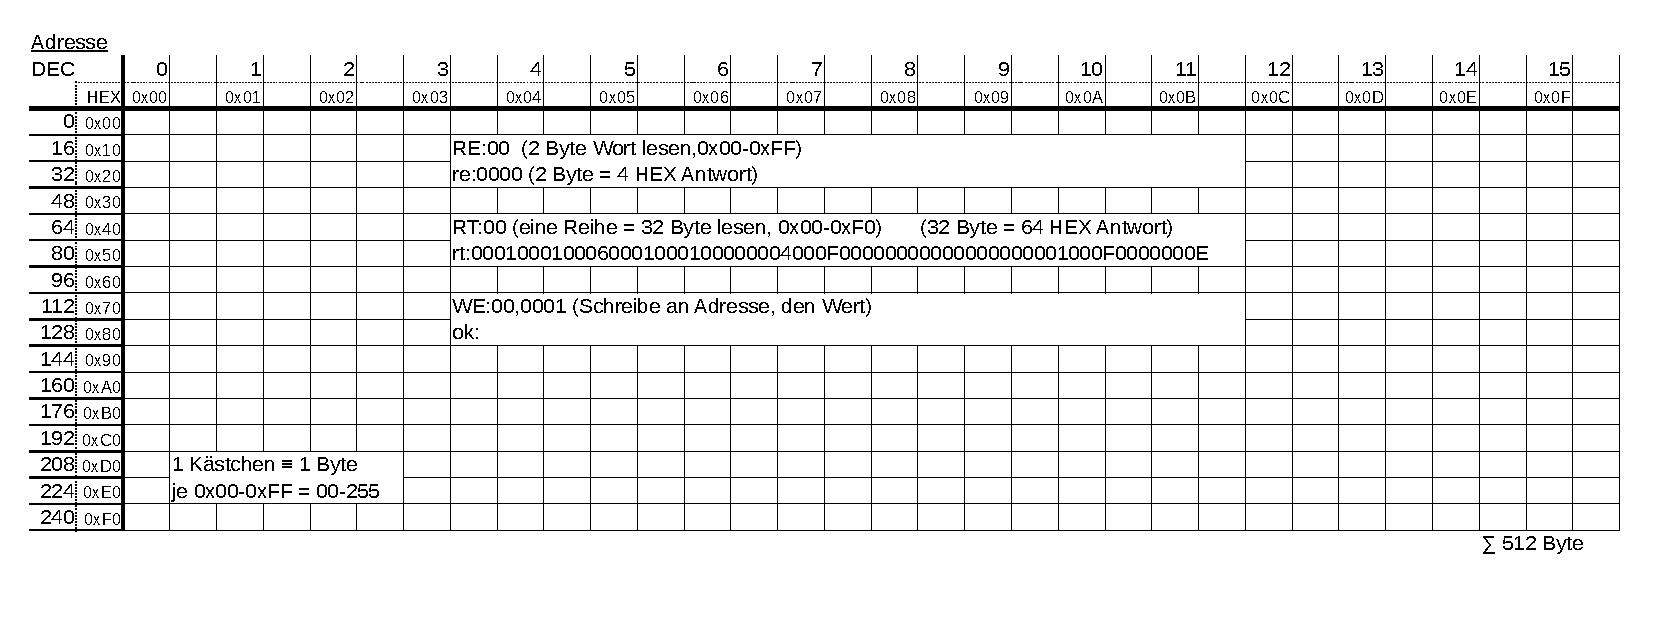
\includegraphics[scale=0.7,trim={0 1.1cm 0 0},clip]{images/chapter_5/Speicher-Schema-Jura-EEPROM}}\\%
    \subfigure[RAM]{\label{subfig:RAM}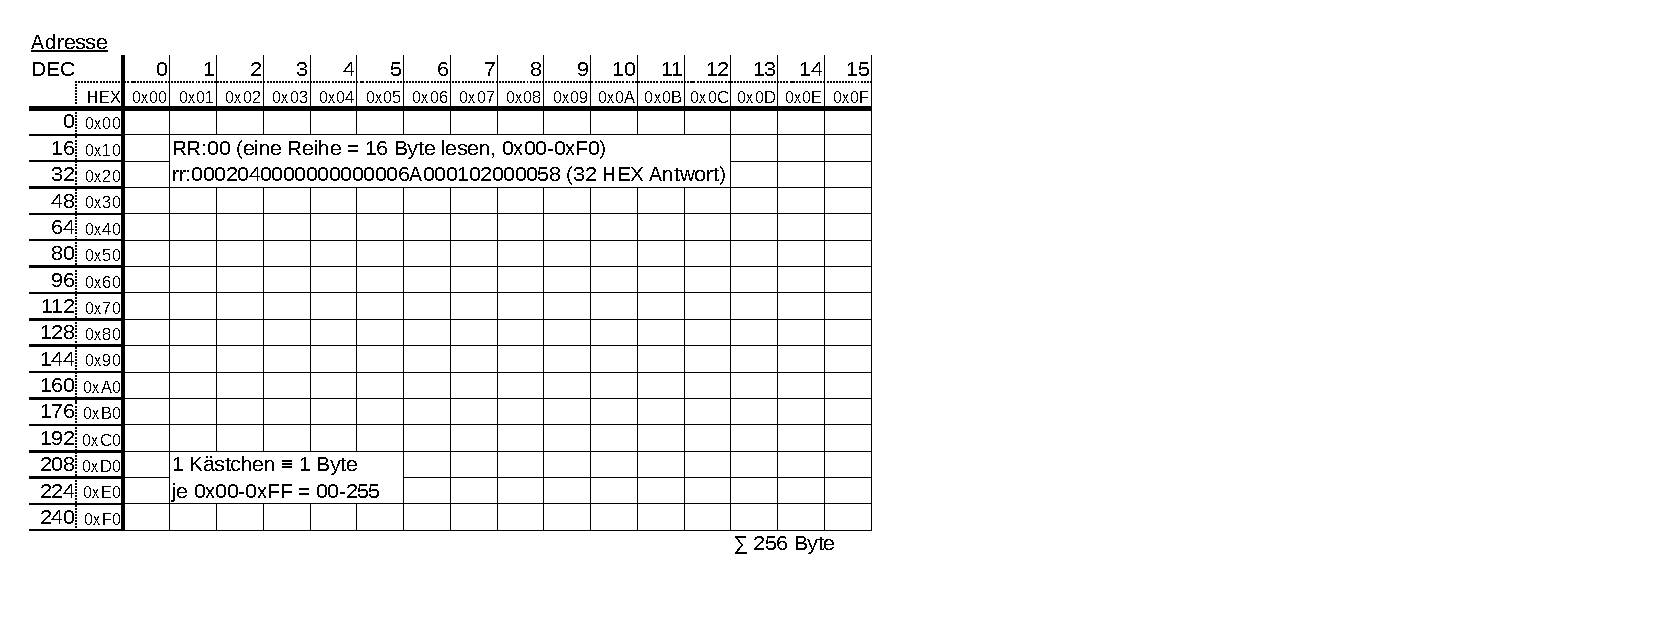
\includegraphics[scale=0.7,trim={0 1.1cm 0 0},clip]{images/chapter_5/Speicher-Schema-Jura-RAM}}%
    \caption{Schematische Darstellung des Speichers vom Kaffeevollautomaten}
    \label{fig:Speicherschema}
\end{sidewaysfigure}

\begin{sidewaystable}
  \footnotesize\centering
  \begin{tabular}[htp]{llllllllll}
  \THc{1}{l}{Funktion} &
  \THc{1}{c}{\rotatebox{50}{Maschine an}} &
  \THc{1}{c}{\rotatebox{50}{Schale fehlt}} &
  \THc{1}{c}{\rotatebox{50}{Schale leeren}} &
  \THc{1}{c}{\rotatebox{50}{Trester leeren}} &
  \THc{1}{c}{\rotatebox{50}{Wasser füllen}} &
  \THc{1}{c}{\rotatebox{50}{Gerät reinigen}} &
  \THc{1}{c}{\rotatebox{50}{Maschine spült}} &
  \THc{1}{c}{\rotatebox{50}{Abschließend spülen}} &
  \THc{1}{c}{\rotatebox{50}{Tassenbeleuchtung}} \\

%
  \TRhc{1}{l}{\textbf{Byte}} &
  \TRhc{1}{l}{\wort{03}} &
  \TRhc{1}{l}{\wort{0E}} &
  \TRhc{1}{l}{\wort{04}} &
  \TRhc{1}{l}{\wort{04}} &
  \TRhc{1}{l}{\wort{04}} &
  \TRhc{1}{l}{\wort{10}} &
  \TRhc{1}{l}{\wort{03}} &
  \TRhc{1}{l}{\wort{0D}} &
  \TRhc{1}{l}{\wort{0F}} \\
  
  Bit &
  \immer{\bitTrue{2}} &
  \immer{\bitTrue{2}} &
  \geteilt{\bitTrue{3}} &
  \bitTrue{5} &
  \geteilt{\bitTrue{3}} &
  \bitTrue{7} &
  \geteilt{\bitTrue{6,3,1}} &
  \bitTrue{3 oder 2} &
  \bitTrue{2 oder 1} \\
  
  \belowbodyrule
%
  \TRhc{1}{l}{\textbf{Byte}} &
  \TRhc{1}{l}{\wort{05}} &
  \TRhc{1}{l}{\wort{16}} &
  \TRhc{1}{l}{\wort{0E}} &
  \TRhc{1}{l}{\wort{0E}} &
  \TRhc{1}{l}{\wort{0E}} &
  \TRhc{1}{l}{\wort{22}} &
  \TRhc{1}{l}{\wort{13}} &
  \TRhc{1}{l}{} &
  \TRhc{1}{l}{} \\
  
  Bit &
  \immer{\bitTrue{5}} &
  \bitFalse{0} &
  \immer{\bitTrue{4}} &
  \bitTrue{5} &
  \immer{\bitTrue{6}} &
  \bitTrue{4} &
  \bitTrue{3,1} &
   &
   \\
  
  \belowbodyrule
%
  \TRhc{1}{l}{\textbf{Byte}} &
  \TRhc{1}{l}{\wort{16}} &
  \TRhc{1}{l}{\wort{29}} &
  \TRhc{1}{l}{\wort{1B}} &
  \TRhc{1}{l}{\wort{80}} &
  \TRhc{1}{l}{\wort{0F}} &
  \TRhc{1}{l}{} &
  \TRhc{1}{l}{\wort{17}} &
  \TRhc{1}{l}{} &
  \TRhc{1}{l}{} \\
  
  Bit &
  \immer{\bitTrue{1}} &
  \immer{\bitFalse{2}} &
  \immer{\bitTrue{1}} &
  \immer{\bitTrue{1,0}} &
  \immer{\bitFalse{4}} &
   &
  \bitTrue{1} &
   &
   \\
  
  \belowbodyrule
%
  \TRhc{1}{l}{\textbf{Byte}} &
  \TRhc{1}{l}{\wort{44}} &
  \TRhc{1}{l}{\wort{69}} &
  \TRhc{1}{l}{\wort{29}} &
  \TRhc{1}{l}{} &
  \TRhc{1}{l}{\wort{4C}} &
  \TRhc{1}{l}{} &
  \TRhc{1}{l}{\wort{62}} &
  \TRhc{1}{l}{} &
  \TRhc{1}{l}{} \\
  
  Bit &
  \immer{\bitTrue{0}} &
  \bitFalse{0} &
  \immer{\bitTrue{6-3}} &
   &
  \geteilt{\bitFalse{0}} &
   &
  \geteilt{\bitTrue{1}} &
   &
   \\
  
  \belowbodyrule
%
  \TRhc{1}{l}{\textbf{Byte}} &
  \TRhc{1}{l}{} &
  \TRhc{1}{l}{} &
  \TRhc{1}{l}{\wort{2B}} &
  \TRhc{1}{l}{} &
  \TRhc{1}{l}{\wort{91}} &
  \TRhc{1}{l}{} &
  \TRhc{1}{l}{} &
  \TRhc{1}{l}{} &
  \TRhc{1}{l}{} \\
  
  Bit &
   &
   &
  \immer{\bitTrue{6-3}} &
   &
  \geteilt{\bitFalse{1}} &
   &
   &
   &
   \\
  
  \belowbodyrule
%
  \TRhc{1}{l}{\textbf{Byte}} &
  \TRhc{1}{l}{\wort{1A}} &
  \TRhc{1}{l}{} &
  \TRhc{1}{l}{} &
  \TRhc{1}{l}{} &
  \TRhc{1}{l}{} &
  \TRhc{1}{l}{} &
  \TRhc{1}{l}{\wort{68}} &
  \TRhc{1}{l}{} &
  \TRhc{1}{l}{} \\
  
  Bit &
  \immer{\bitFalse{2}} &
   &
   &
   &
   &
   &
  \geteilt{\bitTrue{6}} &
   &
   \\
  
  Bit &
  \immer{\bitTrue{1,0}} &
   &
   &
   &
   &
   &
  \geteilt{\bitFalse{5,4}} &
   &
   \\
  \belowbodyrule
  \end{tabular}
  \caption{Speicherpositionen im RAM (1)}
  \label{tbl:RAM1}
\end{sidewaystable}
\begin{sidewaystable}
  \footnotesize\centering
  \begin{tabular}[htp]{lllllllllll}
  \THc{1}{l}{Funktion} &
  \THc{1}{c}{\rotatebox{50}{Filter wechseln}} &
  \THc{1}{c}{\rotatebox{50}{Hahn offen}} &
  \THc{1}{c}{\rotatebox{50}{Teeportion}} &
  \THc{1}{c}{\rotatebox{50}{Dampfbezug}} &
  \THc{1}{c}{\rotatebox{50}{Wasserdampfportion}} &
  \THc{1}{c}{\rotatebox{50}{Pulver füllen}} &
  \THc{1}{c}{\rotatebox{50}{Bohnen füllen}} &
  \THc{3}{c}{\rotatebox{50}{Zubereitung}} \\
  
  \THsub{1}{l}{} &
  \THsub{1}{l}{} &
  \THsub{1}{l}{} &
  \THsub{1}{l}{} &
  \THsub{1}{l}{} &
  \THsub{1}{l}{} &
  \THsub{1}{l}{} &
  \THsub{1}{l}{} &
  \THsub{1}{c}{immer} &
  \THsub{1}{c}{1. Schritt} &
  \THsub{1}{c}{2. Schritt} \\

%
  \TRhc{1}{l}{\textbf{Byte}} &
  \TRhc{1}{l}{\wort{10}} &
  \TRhc{1}{l}{\wort{04}} &
  \TRhc{1}{l}{\wort{03}} &
  \TRhc{1}{l}{\wort{04}} &
  \TRhc{1}{l}{\wort{03}} &
  \TRhc{1}{l}{\wort{04}} &
  \TRhc{1}{l}{\wort{0E}} &
  \TRhc{1}{l}{} &
  \TRhc{1}{l}{} &
  \TRhc{1}{l}{\wort{03}} \\
  
  Bit &
  \bitTrue{5} &
  \geteilt{\bitTrue{3}} &
  \geteilt{\bitTrue{6}} &
  \geteilt{\bitTrue{3}} &
  \geteilt{\bitTrue{3}} &
  \bitTrue{0} &
  \bitTrue{7} &
   &
   &
  \bitTrue{1} \\
  
  \belowbodyrule
%
  \TRhc{1}{l}{\textbf{Byte}} &
  \TRhc{1}{l}{\wort{22}} &
  \TRhc{1}{l}{\wort{0F}} &
  \TRhc{1}{l}{\wort{0B}} &
  \TRhc{1}{l}{\wort{0B}} &
  \TRhc{1}{l}{\wort{0B}} &
  \TRhc{1}{l}{} &
  \TRhc{1}{l}{} &
  \TRhc{1}{l}{} &
  \TRhc{1}{l}{} &
  \TRhc{1}{l}{\wort{0B}} \\
  
  Bit &
  \bitTrue{3} &
  \immer{\bitFalse{6}} &
  \geteilt{\bitFalse{3}} &
  \geteilt{\bitFalse{3}} &
  \geteilt{\bitFalse{3}} &
   &
   &
   &
   &
  \geteilt{\bitFalse{3}} \\
    
  \belowbodyrule
%
  \TRhc{1}{l}{\textbf{Byte}} &
  \TRhc{1}{l}{\wort{F8}} &
  \TRhc{1}{l}{\wort{4C}} &
  \TRhc{1}{l}{\wort{0F}} &
  \TRhc{1}{l}{\wort{13}} &
  \TRhc{1}{l}{\wort{13}} &
  \TRhc{1}{l}{} &
  \TRhc{1}{l}{} &
  \TRhc{1}{l}{} &
  \TRhc{1}{l}{} &
  \TRhc{1}{l}{\wort{17}} \\
  
  Bit &
  \immer{\bitTrue{0}} &
  \geteilt{\bitFalse{0}} &
  \immer{\bitTrue{5}} &
  \bitTrue{2-0} &
  \bitTrue{2,0} &
   &
   &
   &
   &
  \bitTrue{3} \\
  
  \belowbodyrule
%
  \TRhc{1}{l}{\textbf{Byte}} &
  \TRhc{1}{l}{} &
  \TRhc{1}{l}{\wort{4D}} &
  \TRhc{1}{l}{\wort{4C}} &
  \TRhc{1}{l}{\wort{49}} &
  \TRhc{1}{l}{\wort{49}} &
  \TRhc{1}{l}{} &
  \TRhc{1}{l}{} &
  \TRhc{1}{l}{} &
  \TRhc{1}{l}{} &
  \TRhc{1}{l}{\wort{62}} \\
  
  Bit &
   &
  \bitTrue{3,1} &
  \geteilt{\bitFalse{0}} &
  \geteilt{\bitTrue{0}} &
  \geteilt{\bitTrue{0}} &
   &
   &
   &
   &
  \geteilt{\bitTrue{1}} \\
  
  \belowbodyrule
%
  \TRhc{1}{l}{\textbf{Byte}} &
  \TRhc{1}{l}{} &
  \TRhc{1}{l}{} &
  \TRhc{1}{l}{\wort{68}} &
  \TRhc{1}{l}{\wort{4C}} &
  \TRhc{1}{l}{\wort{4C}} &
  \TRhc{1}{l}{} &
  \TRhc{1}{l}{} &
  \TRhc{1}{l}{} &
  \TRhc{1}{l}{} &
  \TRhc{1}{l}{\wort{68}} \\
  
  Bit &
   &
   &
  \geteilt{\bitTrue{6}} &
  \geteilt{\bitFalse{0}} &
  \geteilt{\bitFalse{0}} &
   &
   &
   &
   &
  \geteilt{\bitFalse{5}} \\
  
  \belowbodyrule
%
  \TRhc{1}{l}{\textbf{Byte}} &
  \TRhc{1}{l}{\wort{F9}} &
  \TRhc{1}{l}{} &
  \TRhc{1}{l}{\wort{4D}} &
  \TRhc{1}{l}{} &
  \TRhc{1}{l}{} &
  \TRhc{1}{l}{} &
  \TRhc{1}{l}{} &
  \TRhc{1}{l}{\wort{0A}} &
  \TRhc{1}{l}{\wort{03}} &
  \TRhc{1}{l}{} \\
  
  Bit &
  \bitTrue{7,6,5,4,2} &
   &
  \bitFalse{3,1} &
   &
   &
   &
   &
  \bitTrue{6} &
  \bitTrue{7,4} &
   \\
  
   &
  (\wert{$0_{10} \rightarrow 244_{10}$}) &
   &
  \bitTrue{0} &
   &
   &
   &
   &
  (2-0: "`Kaffee"') &
  (7 nicht manuell) &
   \\
  \belowbodyrule
  \end{tabular}
  \caption{Speicherpositionen im RAM (2)}
  \label{tbl:RAM2}
\end{sidewaystable}

\begin{sidewaysfigure}
  \begin{center}
    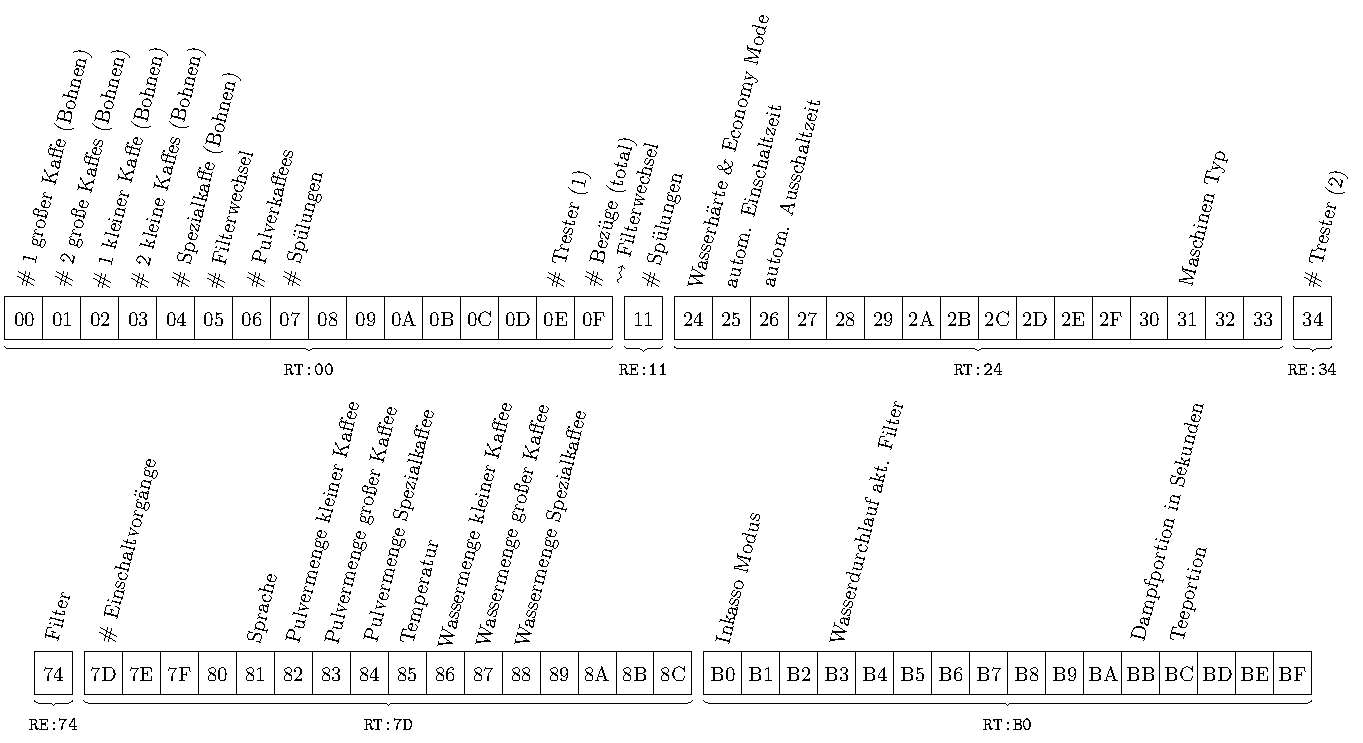
\includegraphics[scale=0.94]{images/chapter_5/API-EEPROM}
    \caption{Abgefragte Speicherstellen für die API im EEPROM (1 Kästchen $\equiv$ 1 Wort)}
    \label{fig:API-EEPROM}
  \end{center}
\end{sidewaysfigure}
\begin{sidewaysfigure}
  \begin{center}
    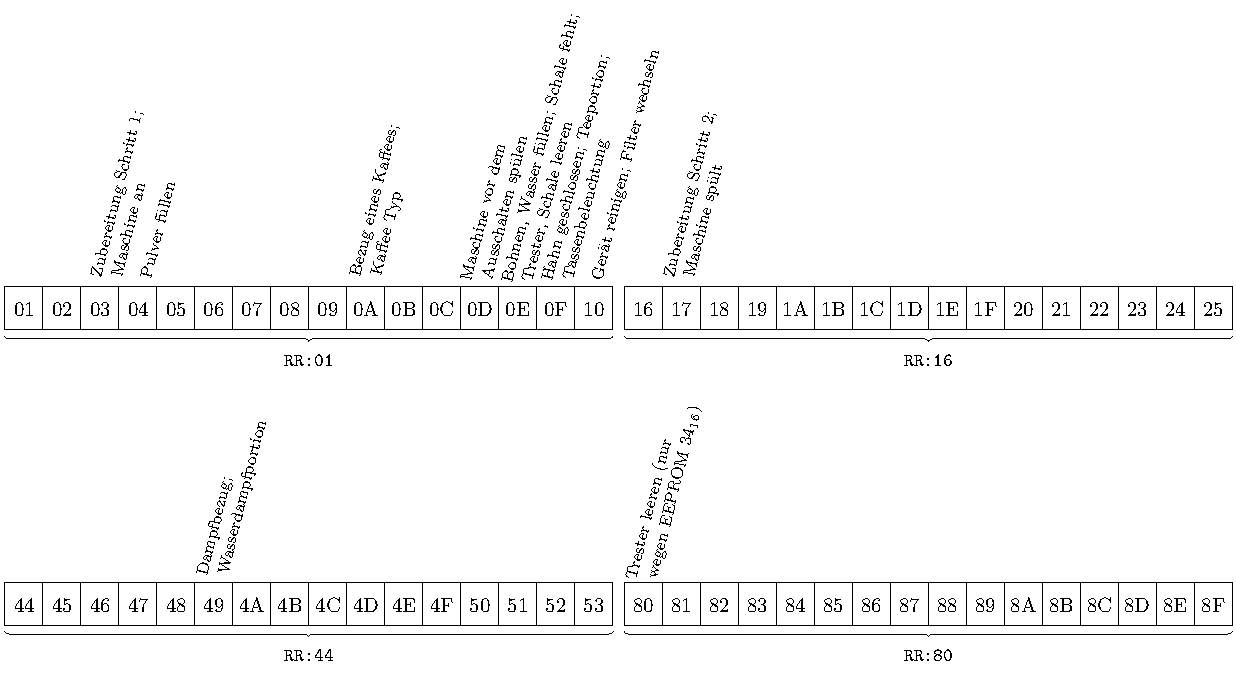
\includegraphics[scale=1]{images/chapter_5/API-RAM}
    \caption{Abgefragte Speicherstellen für die API im RAM (1 Kästchen $\equiv$ 1 Byte)}
    \label{fig:API-RAM}
  \end{center}
\end{sidewaysfigure}

\begin{tuhhtable}
  \newcommand{\display}[1]{\includegraphics[height=2ex]{images/chapter_5/display/#1.png}}
  \footnotesize\centering
  \begin{tabular}[tp]{rrcc   L{1mm}   rrcc}
%
  \THc{3}{c}{ASCII} & \THc{1}{c}{Kaffeevollautomat} &   \TRhc{1}{l}{}   &   \THc{3}{c}{ASCII} & \THc{1}{c}{Kaffeevollautomat} \\
  \THsub{1}{r}{hex} & \THsub{1}{r}{dez} & \THsub{1}{c}{Zeichen} & \THsub{1}{c}{Display} &   \TRhc{1}{l}{}   & \THsub{1}{r}{hex} & \THsub{1}{r}{dez} & \THsub{1}{c}{Zeichen} & \THsub{1}{c}{Display} \\
%
%  \abovebodyrule
%
       & {\tiny 0 – 31} & {\tiny$\ldots$} & {\tiny$\ldots$}   & \TRhc{1}{l}{} &   0x41 & 65            & A                          & A \\\TRc
  0x20 & 32             & Leerzeichen     & Leerzeichen       & \TRhc{1}{l}{} &   0x42 & 66            & B                          & B \\
  0x21 & 33             & !               & \_                & \TRhc{1}{l}{} &   0x43 & 67            & C                          & C \\\TRc
  0x22 & 34             & "               & \display{34}      & \TRhc{1}{l}{} &   0x44 & 68            & D                          & D \\
  0x23 & 35             & \#              & \display{35}      & \TRhc{1}{l}{} &   0x45 & 69            & E                          & E \\\TRc
  0x24 & 36             & \$              & \display{36}      & \TRhc{1}{l}{} &   0x46 & 70            & F                          & F \\
  0x25 & 37             & \%              & \display{37}      & \TRhc{1}{l}{} &   0x47 & 71            & G                          & G \\\TRc
  0x26 & 38             & \&              & \display{38}      & \TRhc{1}{l}{} &   0x48 & 72            & H                          & H \\
  0x27 & 39             & '               & \display{39}      & \TRhc{1}{l}{} &   0x49 & 73            & I                          & I \\\TRc
  0x28 & 40             & (               & \display{40}      & \TRhc{1}{l}{} &   0x4A & 74            & J                          & J \\
  0x29 & 41             & )               & \display{41}      & \TRhc{1}{l}{} &   0x4B & 75            & K                          & K \\\TRc
  0x2A & 42       & \textasteriskcentered & \display{42}      & \TRhc{1}{l}{} &   0x4C & 76            & L                          & L \\
  0x2B & 43             & +               & +                 & \TRhc{1}{l}{} &   0x4D & 77            & M                          & M \\\TRc
  0x2C & 44             & ,               & ,                 & \TRhc{1}{l}{} &   0x4E & 78            & N                          & N \\
  0x2D & 45             & -               & -                 & \TRhc{1}{l}{} &   0x4F & 79            & O                          & O \\\TRc
  0x2E & 46             & .               & .                 & \TRhc{1}{l}{} &   0x50 & 80            & P                          & P \\
  0x2F & 47             & /               & /                 & \TRhc{1}{l}{} &   0x51 & 81            & Q                          & Q \\\TRc
  0x30 & 48             & 0               & 0                 & \TRhc{1}{l}{} &   0x52 & 82            & R                          & R \\
  0x31 & 49             & 1               & 1                 & \TRhc{1}{l}{} &   0x53 & 83            & S                          & S \\\TRc
  0x32 & 50             & 2               & 2                 & \TRhc{1}{l}{} &   0x54 & 84            & T                          & T \\
  0x33 & 51             & 3               & 3                 & \TRhc{1}{l}{} &   0x55 & 85            & U                          & U \\\TRc
  0x34 & 52             & 4               & 4                 & \TRhc{1}{l}{} &   0x56 & 86            & V                          & V \\
  0x35 & 53             & 5               & 5                 & \TRhc{1}{l}{} &   0x57 & 87            & W                          & W \\\TRc
  0x36 & 54             & 6               & 6                 & \TRhc{1}{l}{} &   0x58 & 88            & X                          & X \\
  0x37 & 55             & 7               & 7                 & \TRhc{1}{l}{} &   0x59 & 89            & Y                          & Y \\\TRc
  0x38 & 56             & 8               & 8                 & \TRhc{1}{l}{} &   0x5A & 90            & Z                          & Z \\
  0x39 & 57             & 9               & 9                 & \TRhc{1}{l}{} &   0x5B & 91            & [                          & \display{91} \\\TRc
  0x3A & 58             & :               & :                 & \TRhc{1}{l}{} &   0x5C & 92            & \textbackslash             & \display{92} \\
  0x3B & 59             & ;               & ;                 & \TRhc{1}{l}{} &   0x5D & 93            & ]                          & \display{93} \\\TRc
  0x3C & 60             & <               & <                 & \TRhc{1}{l}{} &   0x5E & 94            & \^{}                       & \display{94} \\
  0x3D & 61             & =               & =                 & \TRhc{1}{l}{} &   0x5F & 95            & \_                         & \display{95} \\\TRc
  0x3E & 62             & >               & >                 & \TRhc{1}{l}{} &   0x60 & 96            & `                          & \display{96} \\
  0x3F & 63             & ?               & ?                 & \TRhc{1}{l}{} &        & {\tiny97-127} & {\tiny a-z \{ | \} $\sim$} & {\tiny$\ldots$} \\\TRc
  0x40 & 64             & @               & \display{64}      & \TRhc{1}{l}{} &        &               &                            &   \\
%
   \belowbodyrule
%
  \end{tabular}
  \caption{Verfügbarer Zeichensatz des Displays}
  \label{tbl:Displaysymbole}
\end{tuhhtable}
